% !TEX program = pdflatex
% !TEX ext =  --interaction=nonstopmode --enable-etex --enable-write18
% !BIB program = none
%%%==============================================================================
%% Copyright 2024-present by Alceu Frigeri
%%
%% This work may be distributed and/or modified under the conditions of
%%
%% * The [LaTeX Project Public License](http://www.latex-project.org/lppl.txt),
%%   version 1.3c (or later), and/or
%% * The [GNU Affero General Public License](https://www.gnu.org/licenses/agpl-3.0.html),
%%   version 3 (or later)
%%
%% This work has the LPPL maintenance status *maintained*.
%%
%% The Current Maintainer of this work is Alceu Frigeri
%%
%% This is version {1.2} {2024/10/22}
%%
%% The list of files that compose this work can be found in the README.md file at
%% https://ctan.org/pkg/tikzdotncross
%%
%%%==============================================================================
\documentclass[10pt]{article}
\RequirePackage[verbose,a4paper,marginparwidth=27.5mm,top=2.5cm,bottom=1.5cm,hmargin={40mm,20mm},marginparsep=2.5mm,columnsep=10mm,asymmetric]{geometry}
\usepackage{codedescribe}
\RequirePackage[inline]{enumitem}
\SetEnumitemKey{miditemsep}{parsep=0ex,itemsep=0.4ex}

\usepackage[american,siunitx,cuteinductors,smartlabels,arrowmos,EFvoltages,betterproportions]{circuitikz}
\usetikzlibrary{math}
\usepackage{tikzdotncross}
\RequirePackage[hidelinks,hypertexnames=false]{hyperref}
\begin{document}
\tstitle{
  author={Alceu Frigeri\footnote{\tsverb{https://github.com/alceu-frigeri/tikzdotncross}}},
  date={\tsdate},
  title={The tikzdotncross Package\break Marking Coordinates and Crossing Paths\break Version \PkgInfo{tikzdotncross}{version}}
  }
  

\begin{typesetabstract}
 
This package offers a few alternative ways for declaring and marking coordinates and drawing a line with ``jumps over'' an already given path, which is a quite common issue when drawing, for instance, Electronics Circuits, e.g. \tsobj[pkg]{CircuiTikZ}.
\end{typesetabstract}

%\tableofcontents

\section{Introduction}
One recurring problem when drawing circuits in general is how to interpret a crossing line. There are many conventions, notably, for the old school (like the author of this) a jump denotes ``non touching lines'' while a simple cross is a connection, more recently (like the past 25 years), the winning convention has been that a dot marks a connection, whilst a simple cross denotes ``non touching lines''. Many, for the sake of staying in the safe side of the wall,  mark a connection with dots and non touching lines with a jump, which is a bit overkill, but at least there is no margin for interpretation errors.

And that's it, this package defines some commands to mark/pin a connection, declaring a coordinate and node at the same spot, for later reference, and a command to draw a line jumping over crossing lines of a pre-existent path.


\section{Package Options}\label{options}
\begin{describelist}{option}
  \describe {pinsize} {pin (circle) size (default: 1.2), in pt.}
  \describe {pinang} {pin angle (default: 45). }
  \describe {pincolor} {pin color (default: blue).}
  \describe {pinlength} {pin length (default: 4), in pt.}
  \describe {coordcolor} {coordinate color (default: red), used if \tsobj{\showcoordstrue}.}
\end{describelist}
 

Those can also be set, middle code, via:
\begin{codedescribe}[code,new=2024/10/22]{\setpindefaults}
\begin{codesyntax}%
\tsmacro{\setpindefaults}{options as above}
\end{codesyntax}
\end{codedescribe}

\section{Declaring and Marking Coordinates/Nodes}\label{coord}
Those are based on some ideas from Redaelli et al. (\tsobj[pkg]{CircuiTikZ}). Main differences: a variable number of parameters (see below) and it always also adds an empty node n\tsobj[marg]{coord}.
\begin{codedescribe}{\showcoordstrue,\shoocoordsfalse}
\begin{codesyntax}%
\tsmacro{\showcoordstrue}{}
\tsmacro{\showcoordsfalse}{}
\end{codesyntax}
These will affect how \tsobj{\ncoord,\dotcoord,\odotcoord} will behave, with \tsobj{\showcoordstrue} a red pin will also be added to the newly defined coordinate/node. The initial state is \tsobj{\showcoordsfalse}. It can be turned on/off as needed.
\end{codedescribe}

\begin{codedescribe}{\ncoord,\pincoord}
\begin{codesyntax}%
\tsobj{\ncoord}\tsverb{(}\tsobj[oarg]{coord}\tsverb{)}
\tsobj{\pincoord}\tsverb{(}\tsobj[oarg,sep={,}]{coord}\tsverb{)}
\tsobj{\pincoord}\tsverb{(}\tsobj[oarg,sep={,}]{coord,color}\tsverb{)}
\tsobj{\pincoord}\tsverb{(}\tsobj[oarg,sep={,}]{coord,color,angle}\tsverb{)}
\tsobj{\pincoord}\tsverb{(}\tsobj[oarg,sep={,}]{coord,color,angle,length}\tsverb{)}
\end{codesyntax}
The \tsobj{\ncoord} always expects a single parameter \tsobj[parg]{coord}. A coordinate named \tsobj[marg]{coord} and node named n\tsobj[marg]{coord} (a ``n'' is added as a prefix) will be created for later use/reference. If \tsobj{\showcoordstrue} is en force, it will also add a pin.

The \tsobj{\pincoord} always draws a pin, besides declaring a coordinate and node as \tsobj{\ncoord}. It expects one to 4 parameters, as listed. If omitted, the default length is 4 (unit: pt), the default angle is -45 (degrees), the default color is blue.
Likewise, if \tsobj{\showcoordstrue}, \tsobj{\coord(name)} is just a short cut for \tsverb{\pincoord(name,red,45)}.
\end{codedescribe}
\begin{tsremark}
  Those defaults can be changed via package options, see \ref{options}, or \tsobj{\setpindefaults}.
\end{tsremark}

\begin{codedescribe}{\dotcoord,\dotpincoord}
\begin{codesyntax}%
\tsobj{\dotcoord}\tsverb{(}\tsobj[oarg]{coord}\tsverb{)}
\tsobj{\dotpincoord}\tsverb{(}\tsobj[oarg,sep={,}]{coord}\tsverb{)}
\tsobj{\dotpincoord}\tsverb{(}\tsobj[oarg,sep={,}]{coord,color}\tsverb{)}
\tsobj{\dotpincoord}\tsverb{(}\tsobj[oarg,sep={,}]{coord,color,angle}\tsverb{)}
\tsobj{\dotpincoord}\tsverb{(}\tsobj[oarg,sep={,}]{coord,color,angle,length}\tsverb{)}
\end{codesyntax}
These are the same as \tsobj{\ncoord} and friends, just adding a dot (a filled in, small circle) at the coordinate.
\end{codedescribe}

\begin{codedescribe}{\odotcoord,\odotpincoord}
\begin{codesyntax}%
\tsobj{\odotcoord}\tsverb{(}\tsobj[oarg]{coord}\tsverb{)}
\tsobj{\odotpincoord}\tsverb{(}\tsobj[oarg,sep={,}]{coord}\tsverb{)}
\tsobj{\odotpincoord}\tsverb{(}\tsobj[oarg,sep={,}]{coord,color}\tsverb{)}
\tsobj{\odotpincoord}\tsverb{(}\tsobj[oarg,sep={,}]{coord,color,angle}\tsverb{)}
\tsobj{\odotpincoord}\tsverb{(}\tsobj[oarg,sep={,}]{coord,color,angle,length}\tsverb{)}
\end{codesyntax}
These are the same as \tsobj{\ncoord} and friends, just adding an open dot (a small circle filled with white) at the coordinate.
\end{codedescribe}



\section{Crossing Paths}\label{pathcross}

\begin{codedescribe}{\pathcross}
\begin{codesyntax}%
\tsobj{\pathcross*}\tsargs[oarg]{cross-name}\tsargs[marg]{coordA,coordB,path-name}\tsargs[oarg]{width}
\end{codesyntax}
This will draw a line from \tsobj[marg]{coordA} to \tsobj[marg]{coordB} ``jumping over'' any pre-existent (soft) path named \tsobj[marg]{path-name}.
First of, the reference path \tsobj[marg]{path-name} has to be defined using the \tsobj[key]{name path} key (\tsobj[key]{name path}=\tsobj[marg]{path-name}).

Then this will ``calculate'' the intersections between the line (defined by the coordinates (\tsobj[marg]{coordA}) and (\tsobj[marg]{coordB}) and the path named \tsobj[marg]{path-name}. At each intersection a coordinate named (\tsobj[oarg]{cross-name}-i) and a node (n\tsobj[oarg]{cross-name}-i) will be defined (i goes from 1 up to the number of crossings detected.) A macro named \tsobj[oarg]{cross-name}T will have the number of crossings found. 

At each intersection a semi-circle will be drawn, and finally a line will be draw connecting \tsobj[marg]{coordA} to \tsobj[marg]{coordB} over all intermediate nodes.

The  star version flips the semi-circles orientation.
\begin{tsremark}
  The default \tsobj[oarg]{cross-name} is ``cross''. It may contain only characters, as any valid \TeX\ macro name. The default \tsobj[oarg]{width} of the semi-circle is 7pt.
\end{tsremark}
\begin{tsremark}
  This is based on the \tsobj[pkg]{tikz} library \tsobj[pkg]{intersetions}, inheriting it's limitations. The main one: It only detects crossings over ``soft paths'', this means, if the line defined by \tsobj[marg]{coordA} and \tsobj[marg]{coordB} crosses over a node, it will, in most cases, miss it (depends on how the node is draw and interacts with the soft path system).
\end{tsremark}
\begin{tsremark}
  When using the crossing coordinates, like (\tsobj[oarg]{cross-name}-i), be aware that in some ill-defined cases, \tsobj[pkg]{intersections} might detect a crossing either at the starting and/or ending points. \tsobj{\pathcross} accounts for that, but you will be left with some extra reference coordinates, either the first one, last one or both.
\end{tsremark}
\end{codedescribe}

%\newpage
\section{Some Examples}
\textbf{\color{red}Note:} In the examples below, the circuit doesn't make much/any sense, it is just a way to show the commands possibilities.

A first example with \tsobj{\showcoordstrue} (showing all coordinates defined with \tsobj{\ncoord}).
\showcoordstrue
\begin{codestore}[crossdemoA]
\resizebox{0.5\textwidth}{!}{
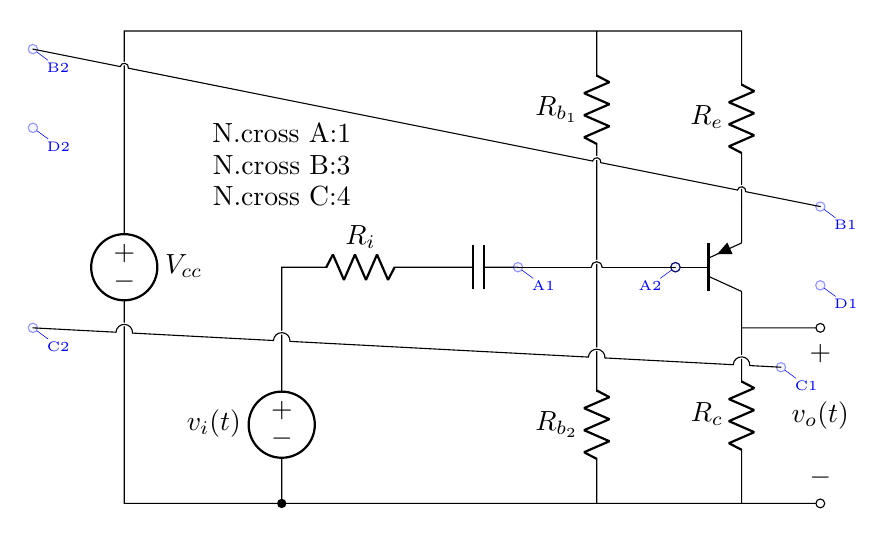
\begin{tikzpicture}
      %% This is the reference, named path
      %%
  		\draw[name path=base circ]
		(0,0) \dotcoord(A) to[V,invert,l=$v_i(t)$] ++(0,2) -- ++(0,1) \ncoord(Y)
      to[R=$R_i$] ++(2,0) 
      to[C] ++(1,0) \pincoord(A1) ++(1,0) \ncoord(B)
       ++(1,0) node[pnp,anchor=B] (T1){}
		(A) -- (A -| B)  to[R=$R_{b_2}$] ++(0,2) \ncoord(Bb) (B) ++(0,1) \ncoord(Cb) to[R=$R_{b_1}$] ++(0,2) \ncoord(C)
		(T1.C) to[R,l_=$R_c$] (T1.C |- A) -- (A)
		(T1.E) to[R,l=$R_e$] (T1.E |- C) -- (C -| A) -- ++(-2,0) \ncoord(X) to[V,l=$V_{cc}$] (X |- A) -- (A)
    (T1.C) -- ++(1,0) node[ocirc]{} \ncoord(k) to[open,v=$v_o(t)$] (k |- A) node[ocirc]{} -- (A)
    (Bb) -- (Cb)
    ;
    %% These are just a few, marked, coords (they could be part of the previous path
    %%
  \path (T1.E)  ++(1,0)      \pincoord(B1)    ++(-10,2)    \pincoord(B2)
        (B1) ++(0,-1)        \pincoord(D1) (B2) ++(0,-1)   \pincoord(D2) 
        (T1.C)  ++(0.5,-0.5) \pincoord(C1) (T1.C) ++(-9,0) \pincoord(C2)
        (T1.B) \odotpincoord(A2,blue,225)
  ;
  %% And that's all, a few crossing lines
  %%
  \pathcross{A1}{A2}{base circ}[4pt] \draw (Y) +(0,1.7) node(){N.cross A:\crossT};
  \pathcross*{B1}{B2}{base circ}[3pt]  \draw (Y) +(0,1.3) node(){N.cross B:\crossT};
  \pathcross*[sec]{C1}{C2}{base circ}[6pt] \draw (Y) +(0,0.9) node(){N.cross C:\secT};
  
\end{tikzpicture}
}
\end{codestore}

\tsdemo*[emph={draw,node,ncoord,pincoord,dotcoord,odotcoord},emph2={pathcross},emph3={name,path},basicstyle={\scriptsize\ttfamily},numbers=left]{crossdemoA}

And the same with \tsobj{\showcoordsfalse}
\showcoordsfalse

\tsresult*[emph={draw,node,ncoord,pincoord,dotcoord,odotcoord},emph2={pathcross},emph3={name,path},basicstyle={\scriptsize\ttfamily},numbers=left]{crossdemoA}

\newpage
As said, the main limitation (derived from how \tsobj[pkg]{intersections} works) is that crossings between the line and nodes might not be detected at all. For example, if someone tries to connect the nodes \tsobj[key]{D1,D2}, it will, unfortunately, fail detecting the node (pnp transistor) entirely:

%\showcoordstrue
%\setpindefaults{coordcolor=cyan,pincolor=red}
\begin{codestore}[crossdemoC]
\resizebox{0.5\textwidth}{!}{
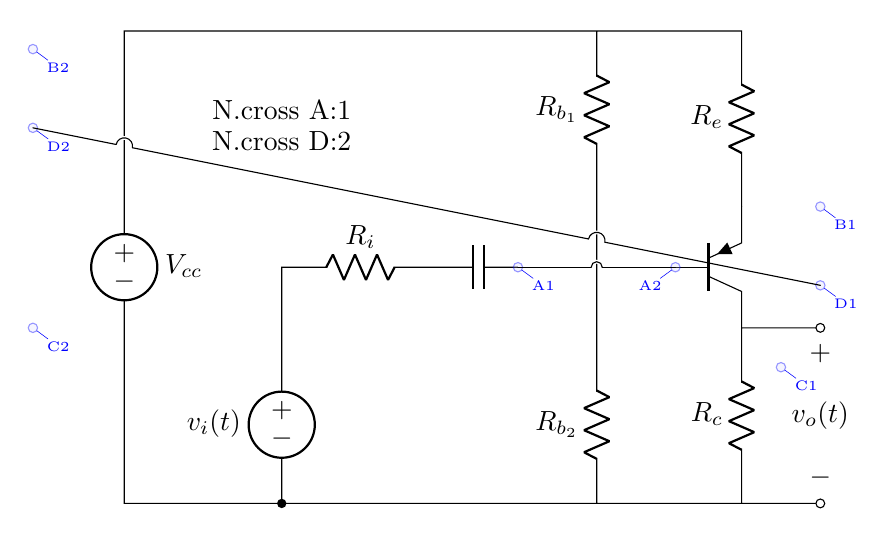
\begin{tikzpicture}
      %% This is the reference, named path
      %%
  		\draw[name path=base circ]
		(0,0) \dotcoord(A) to[V,invert,l=$v_i(t)$] ++(0,2) -- ++(0,1) \ncoord(Y)
      to[R=$R_i$] ++(2,0) 
      to[C] ++(1,0) \pincoord(A1) ++(1,0) \ncoord(B)
       ++(1,0) node[pnp,anchor=B] (T1){}
		(A) -- (A -| B)  to[R=$R_{b_2}$] ++(0,2) \ncoord(Bb) (B) ++(0,1) \ncoord(Cb) to[R=$R_{b_1}$] ++(0,2) \ncoord(C)
		(T1.C) to[R,l_=$R_c$] (T1.C |- A) -- (A)
		(T1.E) to[R,l=$R_e$] (T1.E |- C) -- (C -| A) -- ++(-2,0) \ncoord(X) to[V,l=$V_{cc}$] (X |- A) -- (A)
    (T1.C) -- ++(1,0) node[ocirc]{} \ncoord(k) to[open,v=$v_o(t)$] (k |- A) node[ocirc]{} -- (A)
    (Bb) -- (Cb)
    ;
    %% These are just a few, marked, coords (they could be part of the previous path
    %%
  \path (T1.E)  ++(1,0)      \pincoord(B1)    ++(-10,2)    \pincoord(B2)
        (B1) ++(0,-1)        \pincoord(D1) (B2) ++(0,-1)   \pincoord(D2) 
        (T1.C)  ++(0.5,-0.5) \pincoord(C1) (T1.C) ++(-9,0) \pincoord(C2)
        (T1.B) \pincoord(A2,blue,225)
  ;
  %% And that's all, a few crossing lines
  %%
  \pathcross{A1}{A2}{base circ}[4pt]          \draw (Y) +(0,2) node(){N.cross A:\crossT};
  \pathcross[sec]{D2}{D1}{base circ}[6pt]     \draw (Y) +(0,1.6) node(){N.cross D:\secT};
\end{tikzpicture}
}
\end{codestore}

\tsdemo*[emph={draw,node,ncoord,pincoord,dotcoord,odotcoord},emph2={pathcross},emph3={name,path},basicstyle={\scriptsize\ttfamily},numbers=left]{crossdemoC}


\end{document} 